\section{General modelling theory II}
%------------------------------------------------------------------------------
\begin{frame}{Homework assignment solution: What knowledge is in a globe?}
\begin{columns}[T,onlytextwidth]
\column{0.45\textwidth}
\metroset{block=fill}
\begin{exampleblock}{\footnotesize What information or (abstract) knowledge is embodied or encoded in a globe or Google Maps/Earth? }
    \begin{itemize}\footnotesize
        \item form, rotation, tilt
        \item sizes, distances, topography: continents, bodies of water, mountains, vegetation 
        \item Borders and names of: states, cities, streets, \dots
        \item Places of Interest = POI (shops, traffic, tourism)
        \item Further information: population, traffic data, time zones
    \end{itemize}
\end{exampleblock}
% Aus welchen Gründen bzw. zu welchem Zweck könnten die Modelle zur Originalrepräsentation herangezogen werden?

\column{0.5\textwidth}
\begin{alertblock}{What can it be used for?}
\begin{enumerate}\small
    \item Navigation: plan your travel route
    \item capture borders, distances and locations
    \item explore the earth and its regions, places, etc.
\end{enumerate}
\end{alertblock}

\begin{alertblock}{How? (operating with the model)}
\begin{enumerate}\small
    \item directions / route planning form
    \item turning
    \item zooming in and out
    \item checking or removing certain layers
\end{enumerate}
\end{alertblock}
\end{columns}
\end{frame}

%------------------------------------------------------------------------------
\begin{frame}[allowframebreaks]{3 proporties of a model following Stachowiak}

\metroset{block=fill}
\begin{alertblock}{1)~ Mapping }
\begin{quote} \scriptsize
    „Modelle sind stets Modelle von etwas, nämlich Abbildungen, Repräsentationen natürlicher oder künstlicher Originale, die selbst wieder Modelle sein können.“ 
    %„Originale und Modelle werden hier ausschließlich als Attributklassen gedeutet, die oft die spezielle Gestalt attributiver Systeme erlangen.“ % 131
    „Der Abbildungsbegriff fällt mit dem Begriff der Zuordnung von Modell-Attributen zu Original-Attributen zusammen.“ \parencite[131--132]{stachowiak} % 132
    
    \alert{Models are always models of something, i.e. mappings from, representations of natural or artificial originals, that can be models themselves.}
\end{quote}
\end{alertblock}
\begin{alertblock}{2)~ Reduction}
\begin{quote} \scriptsize
    „Modelle erfassen im allgemeinen nicht alle Attribute des durch sie repräsentierten Originals, sondern nur solche, die den jeweiligen Modellerschaffern und/oder Modelbenutzern relevant scheinen.“ \parencite[132]{stachowiak}
    
    \alert{Models in general capture not all attributes of the original represented by them, but rather only those seeming relevant to their model creators and/ or model users.}
\end{quote}
\end{alertblock}
\framebreak 

\begin{alertblock}{3)~ Pragmatism}
\begin{quote} \scriptsize
    „Eine pragmatisch vollständige Bestimmung des Modellbegriffs hat nicht nur die Frage zu berücksichtigen, \emph{wovon} etwas Modell ist \lbrack{}Abbildungsmerkmal\rbrack{}, sondern auch, \emph{für wen, wann} und \emph{wozu} bezüglich seiner je spezifischen Funktionen es Modell ist.“ \parencite[132]{stachowiak} % 132
    
    \alert{ Models are not uniquely assigned to their originals per se. They fulfill their replacement function \\
    a) for particular – cognitive and/ or acting, model using subjects, \\
    b) within particular time intervals and \\
    c) restricted to particular mental or actual operations.}
\end{quote}
\end{alertblock}

\end{frame}


%------------------------------------------------------------------------------
\begin{frame}{Mapping using attributes}
  \begin{columns}[T,onlytextwidth]
  \metroset{block=fill}
    \column{0.45\textwidth}
    \begin{exampleblock}{\small Attributes versus predicates}
    \begin{quote}  \scriptsize
    %„Originale und Modelle werden hier ausschließlich als Attributklassen gedeutet, die oft die spezielle Gestalt attributiver Systeme erlangen.“ \parencite[131]{stachowiak}
    „\punkti alle Attribute \lbrack{}sind\rbrack{} als primär perzeptiv-kogitative Gebilde wohlzuunterscheiden von ihren sprachlichen -- gesprochenen oder geschriebenen oder sonstwie symbolisierten -- \emph{Artikulationen}.“ \parencite[135]{stachowiak}\smallskip
    
    „Es sei angenommen, daß es zu jeder Attributklasse wenigstens \emph{eine} sie elementweise repräsentierende Prädikatklasse gibt.“ \parencite[137]{stachowiak}
    
    \alert{$\to$ each attribute of the original has a predicate class in the model representing it.}
    \end{quote}
    \end{exampleblock}

    % ----------------------------------------------
    \column{0.5\textwidth}
    \metroset{block=fill}
    \begin{exampleblock}{Attributes = properties}
    \begin{quote}  \scriptsize
    %„Originale und Modelle werden hier ausschließlich als Attributklassen gedeutet, die oft die spezielle Gestalt attributiver Systeme erlangen.“ \parencite[131]{stachowiak}
    „Unter Attributen sind Merkmale und Eigenschaften von Individuen, Relationen zwischen Individuen, Eigenschaften von Eigenschaften, Eigenschaften von Relationen usw. zu verstehen.“ 
    „Hiernach sind einem beliebigen Original stets wohlunterscheidbare, nicht weiter zu zerlegende Teilobjekte zuzusprechen, die potentielle oder tatsächliche Träger von Eigenschaften sind und denen gegebenenfalls eine Relationenstruktur aufgeprägt werden kann.“ \parencite[134]{stachowiak}
    
    \alert{$\to$ properties should ideally be atomic}
    \end{quote}
    \end{exampleblock}
  \end{columns}
  \metroset{block=fill}
    \begin{block}{Mapping = assigning attributes between modell and original}
        \begin{quote}\scriptsize
            „Der Abbildungsbegriff fällt mit dem Begriff der Zuordnung von Modell-Attributen zu Original-Attributen zusammen.“ \parencite[132]{stachowiak}
        \end{quote}
    \end{block}
\end{frame}

%------------------------------------------------------------------------------
\begin{frame}{Mapping in the globe modell}
  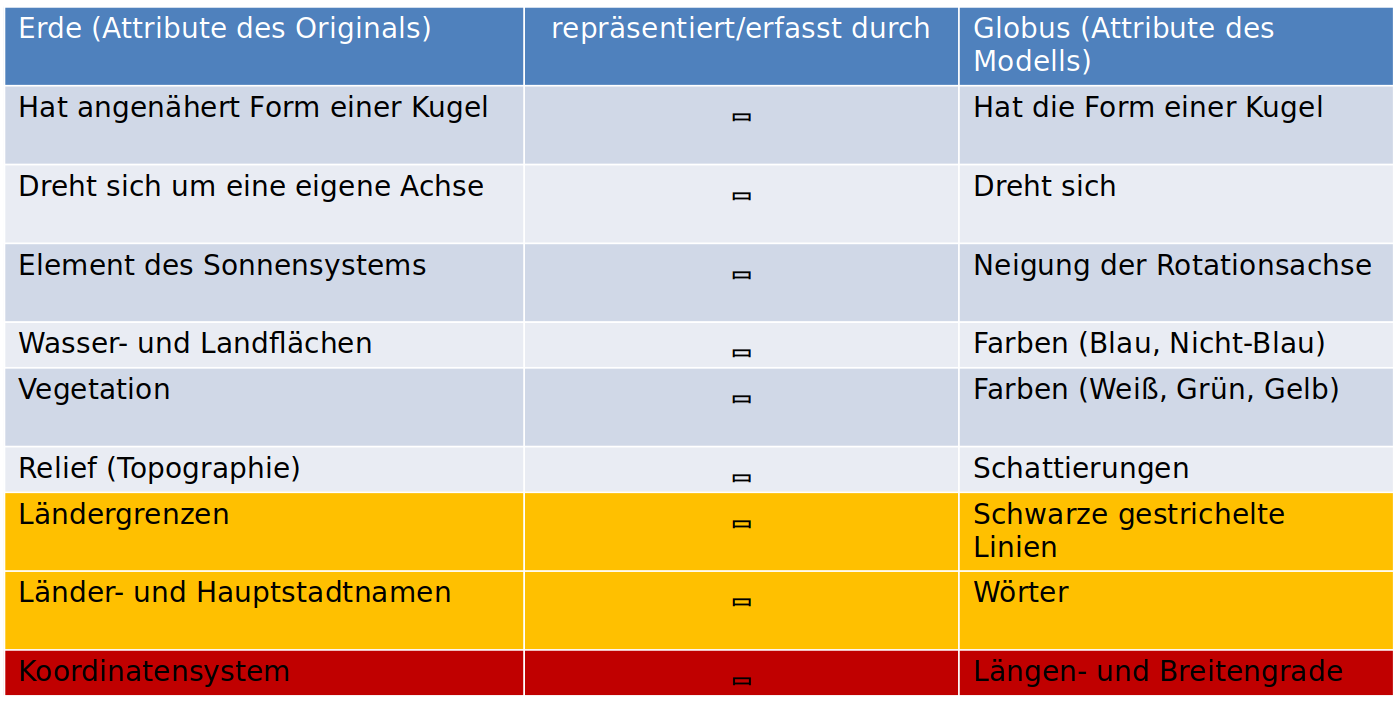
\includegraphics[width=\textwidth]{img/modell-globus.png}  
\end{frame}


%------------------------------------------------------------------------------
\begin{frame}[standout]
    \alert{Discussion:} \small \\  Which originals would you like to model? \\
    Which attributes of the original are to be represented? \\
    What reasons are there for that model?
\end{frame}


%------------------------------------------------------------------------------
\begin{frame}[standout]
    \alert{Reading} for next week: \\
    McCarty, Modelling 
\end{frame}
